	\begin{figure}[!ht]
		\centering
 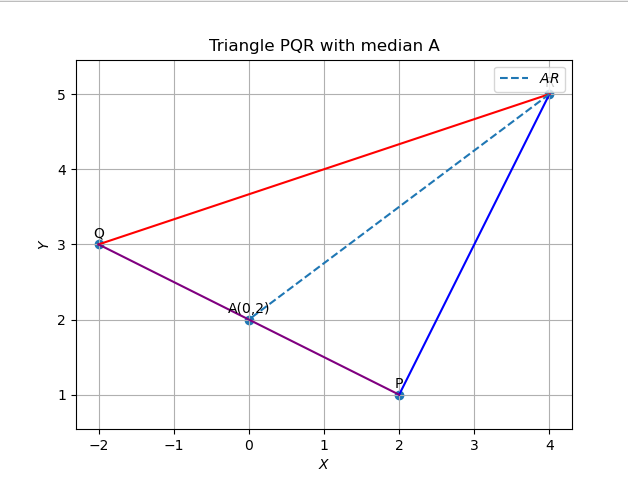
\includegraphics[width=\columnwidth]{chapters/11/10/2/9/figs/line.png}
		\caption{}
		\label{fig:11/10/2/9}
  	\end{figure}
	See Fig. 
		\ref{fig:11/10/2/9}.
Using section formula, the mid point of $PQ$ is
\begin{align}
\vec{A} = \frac{\vec{P} +\vec{Q} }{2}
	= {\myvec{0\\2}}
\end{align} 
So, the direction vector of $AR$ is 
\begin{align}
	\vec{m} ={\vec{R} - \vec{A}}
= \myvec{4 \\ 3}
\\
	\implies \vec{n} = 
 \myvec{3 \\ -4}
\end{align}
which is the normal vector.  Thus,
the equation of the line is 
\begin{align}
	\myvec{3 & -4}\brak{\vec{x} - \vec{R}} = 0
	\\
	\implies 
	\myvec{3 & -4}\vec{x} =8 
\end{align}
